\documentclass[a4paper,12pt]{article}

\usepackage[utf8]{inputenc}
\usepackage[T1]{fontenc}
\usepackage{xcolor,graphicx,fancyhdr,amsmath,amsfonts,amssymb,listings,textcase,siunitx,mathtools}
\usepackage[top=0.6in,bottom=0.7in,right=1in,left=1.25in]{geometry}
\definecolor{black}{RGB}{0,0,0}



% Define parameters
\newcommand{\labnumber}{1}
\newcommand{\labtopic}{\uppercase{Signal generation}}
\newcommand{\subjectname}{Digital Signal Analysis and Processing}

\newcommand{\studentname}{Nimesh Poudel}
\newcommand{\studentid}{KAT078BCT054}
\newcommand{\studentgroup}{B1}
\newcommand{\studentyear}{IV/I}
\newcommand{\submissiondate}{June 2, 2025}

% Page Style
\fancypagestyle{name_roll_page}{
    \fancyhf{}
    \fancyfoot[L]{\texttt{\studentname}}  % Left footer
    \fancyfoot[C]{\texttt{\studentid}}  % Center footer       
    \fancyfoot[R]{\texttt{\thepage}} % Right footer
}

\pagestyle{name_roll_page}

\renewcommand{\headrulewidth}{0pt}
\renewcommand{\footrulewidth}{2pt}
%Font setting
\lstset{upquote=true,showstringspaces=false,stringstyle=\ttfamily,basicstyle=\small}


\begin{document}

% titlepage.tex

\begin{titlepage}
\begin{center}

% Header section
\begin{minipage}{2.5cm}
	\begin{center}
		
\includegraphics[height=2.5cm]{./logo/kec.png}
	\end{center}
\end{minipage}\hfill
\begin{minipage}{10cm}
	\begin{center}
	\Large{\textbf{KATHMANDU ENGINEERING COLLEGE}}\\[0.1cm]
    \small{KALIMATI, KATHMANDU}\\[0.1cm]
    \textbf{TRIBHUVAN UNIVERSITY}
	\end{center}
\end{minipage}\hfill
\begin{minipage}{2.5cm}
	\begin{center}
		
\includegraphics[height=2.5cm]{./logo/tu.jpg}
	\end{center}
\end{minipage}

\vspace{3.5cm}

{\huge \bfseries \uppercase{lab report on} \\[0.5cm] }
{\large \bfseries \subjectname}

\vspace{2.5cm}
{\large \bfseries LAB NO: \labnumber}\\[0.5cm]

\rule{\linewidth}{0.3mm} \\[0.4cm]
{ \huge \bfseries\color{black} \labtopic \\[0.4cm] }
\rule{\linewidth}{0.3mm} \\[3cm]

% Author and supervisor
\begin{tabular}{c @{\hspace{4cm}} c}
    \Large{\textbf{Submitted by:}} & \Large{\textbf{Submitted to:}} \\[1em]
   \large{\MakeUppercase{\studentname}} & \uppercase{Department} \\[0.5em]
    \large{\texttt{\studentid}} & \uppercase{of} \\[0.5em]
    \MakeUppercase{Group: \studentgroup} & \uppercase{Computer} \\[0.5em]
    \MakeUppercase{Year: \studentyear}& \uppercase{Engineering}
\end{tabular}

\vfill

\textbf{\today}

\end{center}
\end{titlepage}



\newpage
\section*{\centering \Huge{\labtopic}}
\section*{Theory}
Signal can be defined as a function of one or more independent variables 
which conveys information about the behavior or nature of some phenomenon. 
It’s examples include electrical signal which is a voltage function of time.
 1-D signals are of two types:
 \begin{itemize}
    \item \textbf{Continuous time signal (CT signal):}
    These signals are defined in every instance of
time under consideration. It is represented as $x(t)$. Ex. Electrical Signal.
    \item \textbf{Discrete time signal (DT signal):}
    These signals are defined only at certain time
instants. Amplitude between two time instances is not defined. It is represented as $x[n]$.
 \end{itemize}
Some basic signals include:
\begin{enumerate}
    \item \textbf{Unit Impulse Signal:} Also known as the Dirac delta function, it is defined as a signal
that is zero at all times except at $t=0$, where it is $1$ (in DT) and $\infty$ (in CT).\\
    For DT:
    \[\delta[n] := \begin{cases}
        1 & \text{if } n = 0\\
        0 & \text{Otherwise}
    \end{cases}\]
    For CT:
    \[\delta(t) := \begin{cases}
        \infty & \text{if } t = 0\\
        0 & \text{Otherwise}
    \end{cases}\]


    \item \textbf{Unit Step Signal:} This signal is $0$ for negative time and $1$ for non negative time.
    \[\theta(t) := \begin{cases}
        0 & \text{if }t < 0\\
        1 & \text{if }t \geq 0
    \end{cases}\]

    \item \textbf{Unit Ramp Signal:} A ramp signal increases linearly with time.
    \[R(t) := \begin{cases}
        0 & \text{if } t \leq 0\\
        t & \text{if } t > 0 
    \end{cases}\]

\item \textbf{Signum Signal:} This signal indicates the sign of a number, returning $-1$ for negative inputs, $0$ at zero, and $1$ for positive inputs.
    \begin{center}
    \begin{minipage}{0.45\linewidth}
    \[
        \text{sgn}(t) := \begin{cases}
            -1 & \text{if } t < 0 \\
            0 & \text{if } t = 0 \\
            1 & \text{if } t > 0
        \end{cases}
    \]
    \end{minipage}
    OR,
    \hfill
    \begin{minipage}{0.45\linewidth}
        \[
            \text{sgn}(t) := \begin{cases}
            0 & \text{if } t = 0 \\
            \dfrac{t}{|t|} & \text{if } t \neq 0
        \end{cases}
        \]
    \end{minipage}
    \end{center}
\item \textbf{Sinusoidal Signal:} A periodic waveform described by sine or cosine functions. 
    \begin{center}
        \begin{minipage}{0.45\linewidth}
            \[x(t) = A \sin(\omega t)\]
        \end{minipage}
        \begin{minipage}{0.45\linewidth}
            \[y(t) = A \cos(\omega t)\]
        \end{minipage}
    \end{center}

\item \textbf{Rectangular Signal:} This signal has a constant amplitude for a fixed interval and is zero elsewhere.
    \[\text{rect}\left(\dfrac{t}{a}\right) = \Pi\left(\dfrac{t}{a}\right) := \begin{cases}
        0,&\text{if } \left\lvert t \right\rvert > \frac{a}{2}\\
        1,&\text{if } \left\lvert t \right\rvert \leq \frac{a}{2}
    \end{cases}\]

\item \textbf{Sinc funcion:} 
    In mathematics, the historical unnormalized sinc function is defined as,
        \[\text{sinc}(t) := \begin{cases}
            1&\text{if } t = 0\\
            \dfrac{\sin(t)}{t}&\text{if } t \neq 0
        \end{cases}\]
        In digital signal processing and information theory, the normalized sinc function is commonly defined as,
        \[\text{sinc}(t) := \begin{cases}
            1&\text{if } t = 0\\
            \dfrac{\sin(\pi t)}{\pi t}&\text{if } t \neq 0
        \end{cases}\]

\end{enumerate}
\newpage
\section*{\centering PROGRAMS}
\subsection*{Unit Impilse Signal}
    \lstinputlisting[language=Octave]{code/unit_impulse.m}
    \begin{figure}[h]
        \centering
        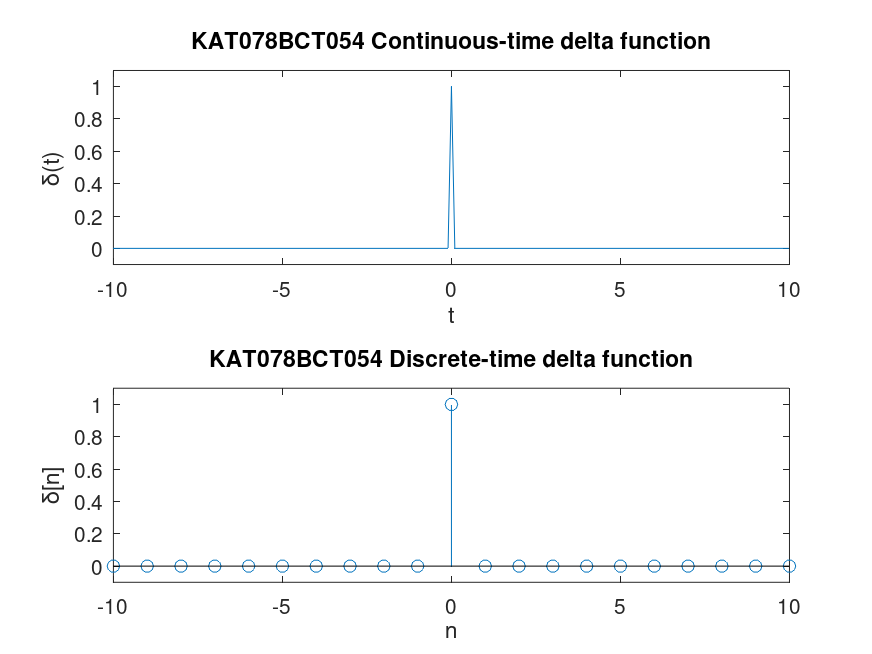
\includegraphics[width=0.7\linewidth]{figures/unit_impulse.png}
        \caption{Unit Impulse Signal}
        \label{unit_impulse}
    \end{figure}
\newpage
\subsection*{Unit Step Signal}
    \lstinputlisting[language=Octave]{code/unit_step.m}
    \begin{figure}[ht]
        \centering
        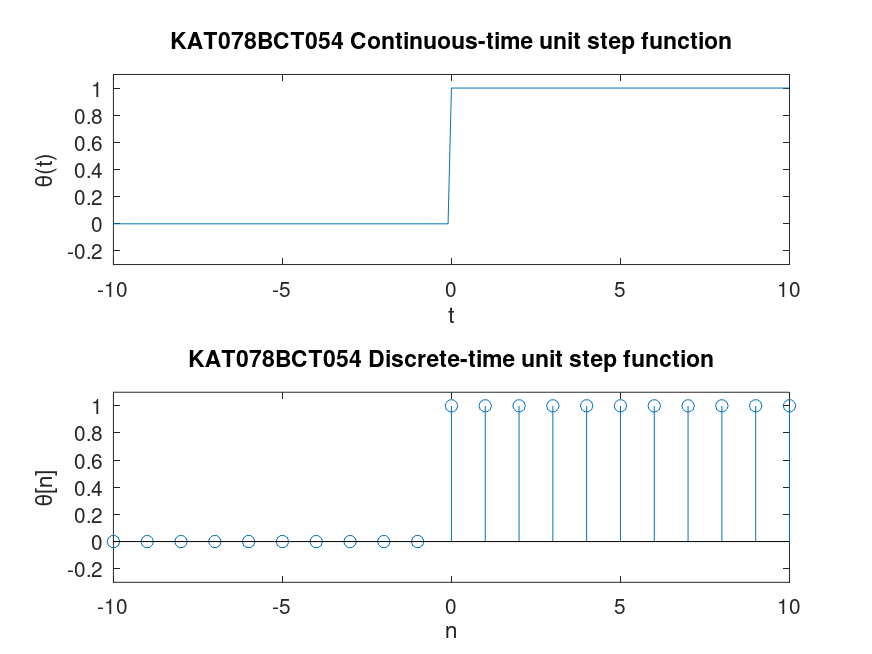
\includegraphics[width=0.7\linewidth]{figures/unit_step.png}
        \caption{Unit Step Signal}
        \label{unit_step}
    \end{figure}
\newpage
\subsection*{Ramp Signal}
    \lstinputlisting[language=Octave]{code/ramp.m}
    \begin{figure}[h]
        \centering
        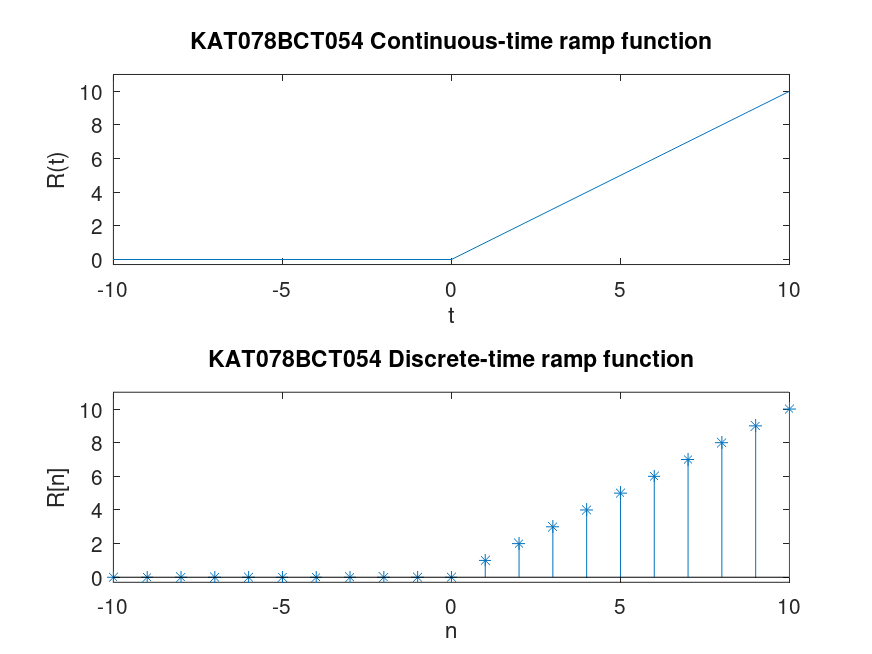
\includegraphics[width=0.7\linewidth]{figures/ramp.png}
        \caption{Ramp Signal}
        \label{ramp}
    \end{figure}
\newpage
\subsection*{Signum Signal}
    \lstinputlisting[language=Octave]{code/sgn.m}
    \begin{figure}[h]
        \centering
        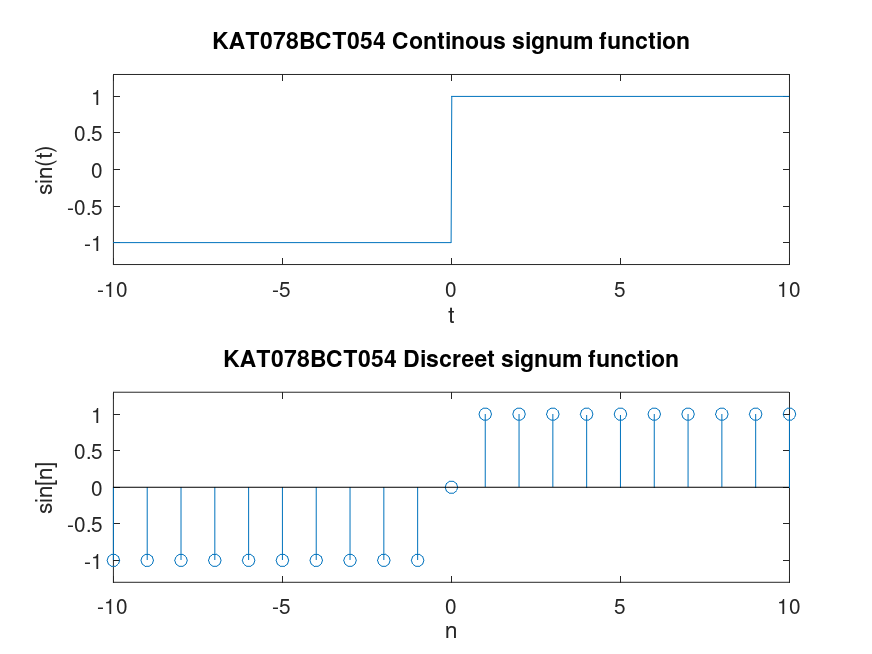
\includegraphics[width=0.7\linewidth]{figures/sgn.png}
        \caption{Signum Signal}
        \label{sgn}
    \end{figure}
\newpage
\subsection*{Rectangular Signal}
    \lstinputlisting[language=Octave]{code/rect.m}
    \begin{figure}[h]
        \centering
        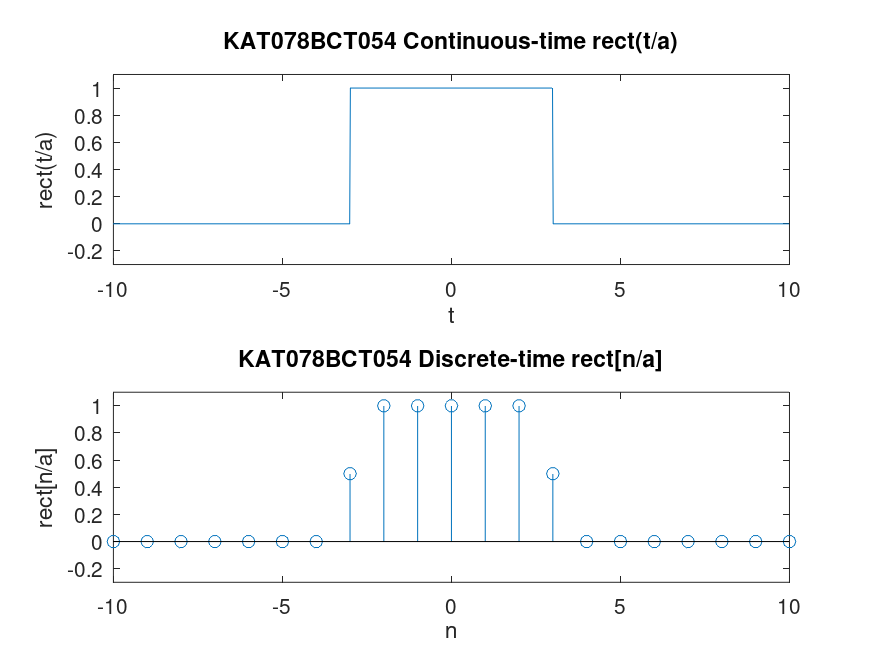
\includegraphics[width=0.6\linewidth]{figures/rect.png}
        \caption{Rectangular Signal}
        \label{rect}
    \end{figure}
\newpage
\subsection*{Sin Signal}
    \lstinputlisting[language=Octave]{code/sine.m}
    \begin{figure}[h]
        \centering
        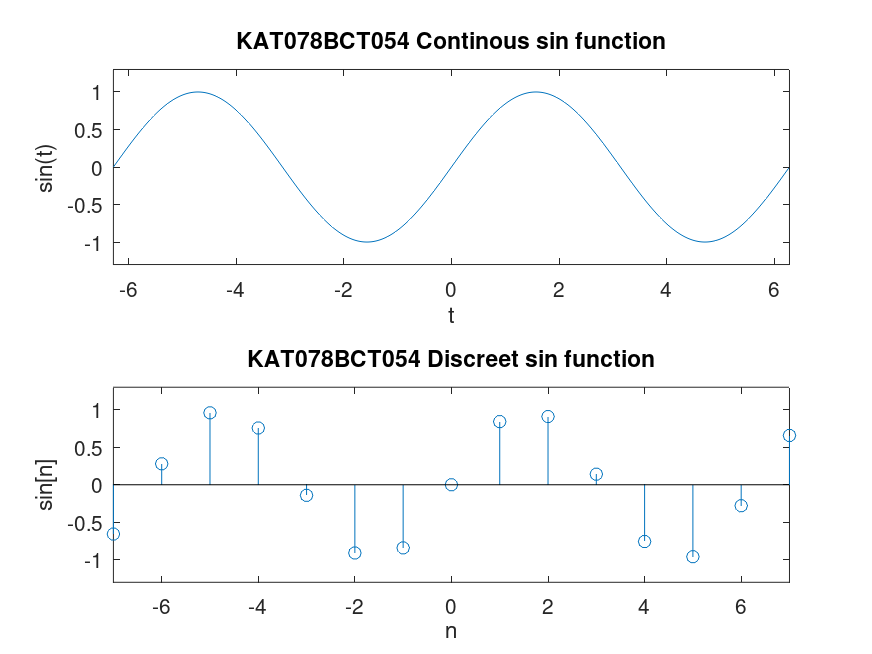
\includegraphics[width=0.7\linewidth]{figures/sin.png}
        \caption{Sin Signal}
        \label{sin}
    \end{figure}
\newpage
\subsection*{Sinc Signal}
    \lstinputlisting[language=Octave]{code/sinc.m}
    \begin{figure}[h]
        \centering
        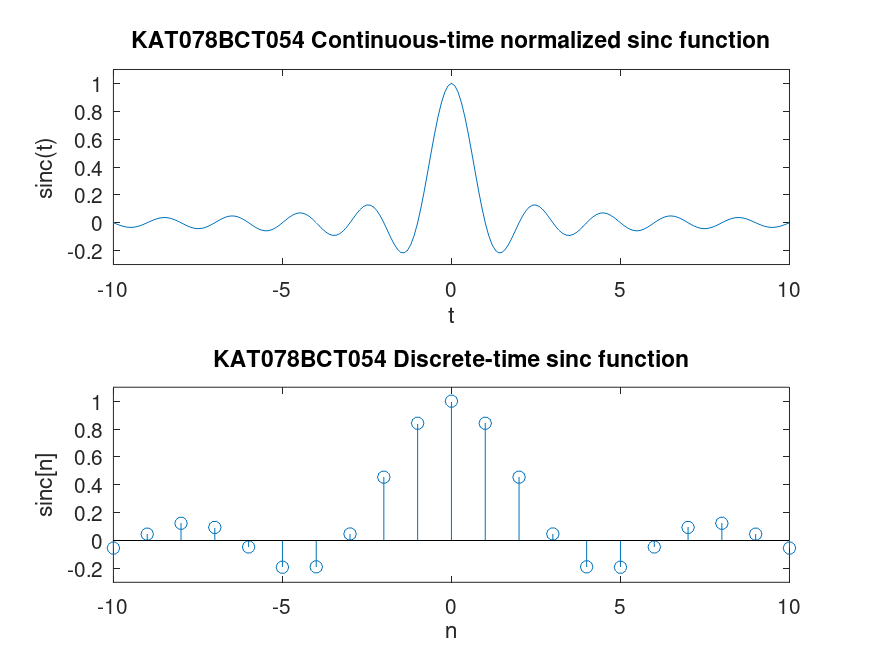
\includegraphics[width=0.7\linewidth]{figures/sinc.png}
        \caption{Sinc Signal}
        \label{sinc}
    \end{figure}
\newpage
\subsection*{Discussion}
During this lab, we implemented MATLAB scripts to generate various fundamental signals. We observed that the continuous signals were plotted using smooth curves, while discrete signals were plotted using discrete data points, providing a clear representation of sampled data. 
\subsection*{Conclusion}
Hence, we successfully generated various basic signals using MATLAB. Through this, we visualized the behavior of fundamental signals that are essential in the analysis and design of communication systems, control systems, and signal processing applications.
\end{document}